\documentclass[border=4pt]{standalone}
\usepackage{tikz}
\usetikzlibrary{arrows.meta,positioning,calc,fit,backgrounds,patterns,shapes.geometric}
\usepackage{amsmath,amssymb}
\usepackage{mathptmx}
\definecolor{lost}{HTML}{C2362D}
\definecolor{kept}{HTML}{17875A}
\definecolor{evid}{HTML}{3056D3}
\definecolor{ink}{HTML}{1D1D1F}
\definecolor{muted}{HTML}{6E6E73}
\tikzset{
  box/.style={draw=ink!70, rounded corners=2pt, align=center, fill=white, inner sep=4pt, font=\footnotesize},
  arr/.style={-{Stealth[length=2mm]}, draw=ink!70, line width=0.6pt},
  grp/.style={draw=muted!60, dashed, rounded corners=4pt, inner sep=7pt},
  lossbox/.style={draw=lost!80, fill=lost!6, text=lost!85!black, rounded corners=2pt, align=left, font=\footnotesize, inner sep=4pt},
  fixbox/.style={draw=kept!80, fill=kept!7, text=kept!65!black, rounded corners=2pt, align=left, font=\footnotesize, inner sep=4pt},
  dec/.style={diamond, aspect=2.2, draw=ink!70, fill=evid!6, align=center, font=\footnotesize, inner sep=1.5pt},
  lbl/.style={font=\footnotesize\bfseries, text=ink},
}

\begin{document}
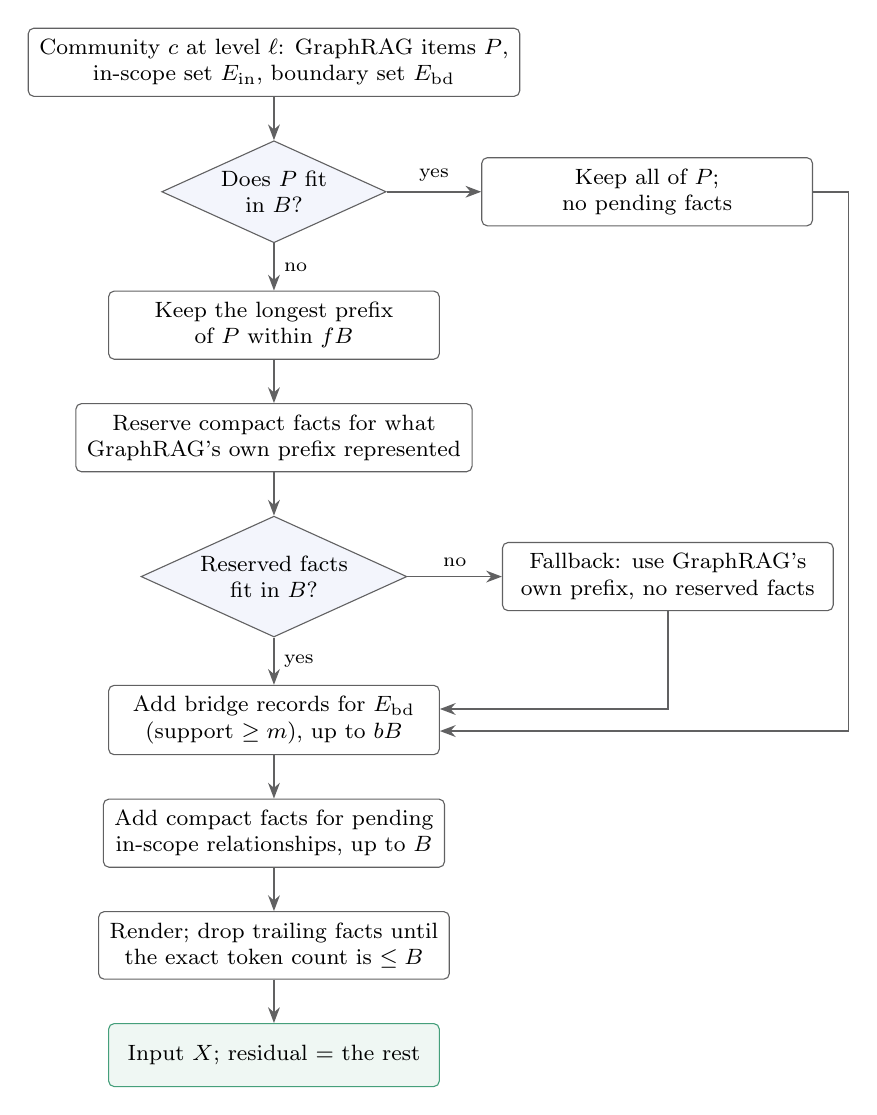
\begin{tikzpicture}[node distance=0.55cm]
\tikzset{st/.style={box, minimum width=4.2cm, minimum height=0.8cm}}
\node[st] (s0) {Community $c$ at level $\ell$: GraphRAG items $P$,\\in-scope set $E_{\mathrm{in}}$, boundary set $E_{\mathrm{bd}}$};
\node[dec, below=of s0] (d1) {Does $P$ fit\\in $B$?};
\node[st, right=1.2cm of d1] (fit) {Keep all of $P$;\\no pending facts};
\node[st, below=0.6cm of d1] (cut) {Keep the longest prefix\\of $P$ within $fB$};
\node[st, below=of cut] (res) {Reserve compact facts for what\\GraphRAG's own prefix represented};
\node[dec, below=of res] (d2) {Reserved facts\\fit in $B$?};
\node[st, right=1.2cm of d2] (fb) {Fallback: use GraphRAG's\\own prefix, no reserved facts};
\node[st, below=0.6cm of d2] (br) {Add bridge records for $E_{\mathrm{bd}}$\\(support $\ge m$), up to $bB$};
\node[st, below=of br] (cf) {Add compact facts for pending\\in-scope relationships, up to $B$};
\node[st, below=of cf] (ck) {Render; drop trailing facts until\\the exact token count is $\le B$};
\node[st, below=of ck, fill=kept!7, draw=kept!80] (out) {Input $X$; residual $=$ the rest};
\draw[arr] (s0) -- (d1);
\draw[arr] (d1) -- node[above, font=\scriptsize] {yes} (fit);
\draw[arr] (d1) -- node[right, font=\scriptsize] {no} (cut);
\draw[arr] (cut) -- (res); \draw[arr] (res) -- (d2);
\draw[arr] (d2) -- node[above, font=\scriptsize] {no} (fb);
\draw[arr] (d2) -- node[right, font=\scriptsize] {yes} (br);
\draw[arr] (fit.east) -- ++(0.45,0) |- ($(br.east)+(0,-0.14)$);
\draw[arr] (fb.south) |- ($(br.east)+(0,0.14)$);
\draw[arr] (br) -- (cf); \draw[arr] (cf) -- (ck); \draw[arr] (ck) -- (out);
\end{tikzpicture}
\end{document}
